%%%%%%%%%%%%%%%%%%%%%%%%%%%%%%%%%%%%%%%%%
%                                       %
% Latex File for the Figures and Tables %
%                                       %
%%%%%%%%%%%%%%%%%%%%%%%%%%%%%%%%%%%%%%%%%


\documentclass[journal, onecolumn]{IEEEtran}

\RequirePackage{times}
\usepackage{epsfig}
\DeclareMathAlphabet{\mathtsl}{OT1}{ptm}{m}{sl}

\usepackage{helvet}
\usepackage{enumerate}
\usepackage{amsmath}
\usepackage{amsfonts}
\usepackage{graphicx}
\usepackage{multirow}
\usepackage{subfig}
\usepackage{comment}
\usepackage{mathtools}
\usepackage{color}


\begin{document}

%%%%%%%%%%%% Macro definitions %%%%%%%%%%%%%%%%%%%%%%%%%%%%%%%%%
\newtheorem{theorem}{Theorem}
\newtheorem{lemma}{Lemma}
\newtheorem{corollary}{Corollary}
\newtheorem{Definition}{Definition}[section]
\newtheorem{Example}{Example}[section]
\newtheorem{Lemma}{Lemma}[section]
%%
\newcommand{\beq}{\begin{equation}}
\newcommand{\eeq}{\end{equation}}
\newcommand{\ov}{\overline}
\newcommand{\xor}{\bigoplus}
%% Tabs
\def\tabnote#1{{\small{#1}}}
%% Algorithm
\def\algorithm{\bgroup\obeylines\obeyspaces\def\ {\quad}
\footnotesize\tt\leftskip=1pc\vskip4pt\relax}
\def\endalgorithm{\vskip4pt\egroup}
%% Line spacing
\newcommand{\ls}[1]
    {\dimen0=\fontdimen6\the\font
     \lineskip=#1\dimen0
     \advance\lineskip.5\fontdimen5\the\font
     \advance\lineskip-\dimen0
     \lineskiplimit=.9\lineskip
     \baselineskip=\lineskip
     \advance\baselineskip\dimen0
     \normallineskip\lineskip
     \normallineskiplimit\lineskiplimit
     \normalbaselineskip\baselineskip
     \ignorespaces
    }
%% Bibliography related
\def\BibTeX{{\rm B\kern-.05em{\sc i\kern-.025em b}\kern-.08em1
    T\kern-.1667em\lower.7ex\hbox{E}\kern-.125emX}}

\setcounter{page}{1}

%%%%%%%%%%% Figures begin %%%%%%%%%%%%%%%%%%%%%%%%%%%

\begin{figure*}[p]
\centerline{
\includegraphics[scale=0.5]{../figures/2bitmultiplier_gates.pdf}}
\caption{}
\label{fig:mul2bit}
\end{figure*}

\clearpage

\begin{figure*}[p]
\begin{align*}
f_1: c_0+a_0 \cdot b_0, \ lm=c_0; ~~~f_2: c_1+a_0 \cdot b_1, \ lm=c_1 \nonumber \\
f_3: c_2+a_1 \cdot b_0, \ lm=c_2; ~~~f_4: c_3+a_1 \cdot b_1, \ lm=c_3 \nonumber \\
f_5: r_0+c_1 + c_2 , \ lm=r_0; ~~~f_6: z_0+c_0 + c_3, \ lm=z_0\nonumber
\end{align*}
\vspace{-0.35in}
\begin{center}
$f_7: z_1+r_0 + c_3, \ lm=z_1$ % \nonumber 
\end{center}
\caption{}
\label{fig:rel_prime_lt}
\end{figure*}

\clearpage

\begin{figure*}[p]
\centering
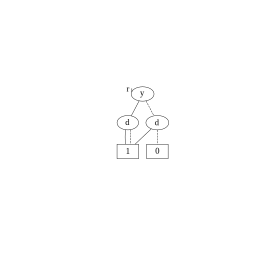
\includegraphics[scale=1]{../figures/r1_clean.pdf}
\label{r1}
\caption{}
\end{figure*}

\clearpage

\begin{figure*}[p]
\centering
\includegraphics[scale=0.40]{../figures/Chain_Or_Gates.pdf}
\label{ChainOrGate}
\caption{}
\end{figure*}

\clearpage

\begin{figure*}[p]
\centering
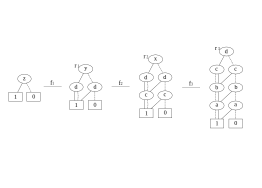
\includegraphics[scale=1.4]{../figures/red_steps.pdf}
\caption{}
\label{red_steps}
\end{figure*}

\clearpage

\begin{figure*}[p]
\centering
\includegraphics[scale=1]{../figures/mod2sumfig_new_1.pdf}
\caption{}
\label{mod2sumfig}
\end{figure*}

\clearpage

\begin{figure*}[p]
\centering
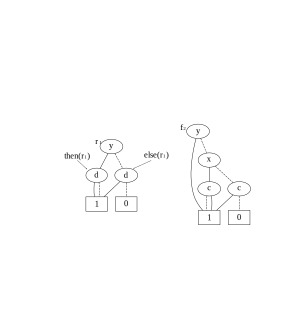
\includegraphics[scale=1]{../figures/r1_f2.pdf}
\caption{}
\label{f2}
\end{figure*}

\clearpage

\begin{figure*}[p]
\centering
\includegraphics[scale=0.34]{../figures/new_mmcircuit.pdf}
\caption{}
\label{montfig}
\end{figure*}

\clearpage

\begin{figure*}[p]
\centering
\includegraphics[scale=0.4]{../figures/2-bit-mult_flipped.pdf}
\caption{}
\label{intmult}
\end{figure*}

\clearpage

%%%%%%%%%%%%%%%%%%%%%%%%%%%%%%%%%%%%%%%%%%%%%%%%%%%%%
%                                                  %      
%                  Tables                          %
%                                                  %
%%%%%%%%%%%%%%%%%%%%%%%%%%%%%%%%%%%%%%%%%%%%%%%%%%%%%

\begin{center}

\begin{table}[ht!]
\centering
\caption{}
\label{masmmsyn}
\begin{tabular}{| c | c || c | c | c | c | c | c | c |} \hline
\multirow{2}{*}{$\boldsymbol{k}$}&\multirow{2}{*}{\textbf{\#Gates}}&\multirow{2}{*}{\textbf{F4~\cite{pruss:tcad}}}& \multirow{2}{*}{\textbf{\#T}}&\multirow{2}{*}{\textbf{~\cite{cunxi:aspdac17}(P)}}& \multicolumn{2}{ c |}{\textbf{PB}}&\multicolumn{2}{ c |}{\textbf{ZR}}\\ \cline{6-9}
&&&&&\textbf{(P)}&\textbf{(S)}&\textbf{(P)}&\textbf{(S)} \\ \hline
64 &11.5K&1.3&20& 3.70&3.60& 2.21&0.73 &\textbf{0.27}\\ \hline 
128 &46K&9.89&20&27.54 &23.99&16.76& 5.08 &\textbf{1.63}\\ \hline 
163 &73.5K&32.61&20& 55.96&48.67&33.72&  11.41&\textbf{3.11}\\ \hline 
233 &122K&86.30& 20&127.61&112.96 &77.23& 21.77&\textbf{3.63}\\ \hline
283 &193K&274.68& 20&253.05&227.77&157.45& 49.89&\textbf{11.41}\\ \hline
409 &386K&2,528.5& 10&716.80 &659.64&426.92& 163.52&\textbf{17.68}\\ \hline
571* &1.6M & TO &3 & 5,331&CR&CR&2,126.7& \textbf{566.4}\\ \hline
\end{tabular}
\end{table}

\end{center}

\clearpage

\begin{center}

\begin{table}[ht!]
\centering
\caption{}
\label{montmmsyn}
\begin{tabular}{| c | c || c | c | c | c | c | c | c |} \hline
\multirow{2}{*}{$\boldsymbol{k}$}&\multirow{2}{*}{\textbf{\#Gates}}&\multirow{2}{*}{\textbf{F4~\cite{pruss:tcad}}}& \multirow{2}{*}{\textbf{\#T}}&\multirow{2}{*}{\textbf{~\cite{cunxi:aspdac17}(P)}}& \multicolumn{2}{ c |}{\textbf{PB}}&\multicolumn{2}{ c |}{\textbf{ZR}}\\ \cline{6-9}
&&&&&\textbf{(P)}&\textbf{(S)}&\textbf{(P)}&\textbf{(S)} \\ \hline
64 &9.5K&16.29&20&10.69&6.27&9.22& \textbf{3.75} & 8.37\\ \hline 
128 &35K&621.90&20& 36.19&28.93&34.59&  \textbf{13.76}&24.73\\ \hline 
163 &56.5K&2,608.4&20&204.94 &167.73&335.2&  \textbf{141.68}&321.60\\ \hline 
233 &111K&385.92& 20&132.51& 119.77&99.36 &42.16&\textbf{31.88}\\ \hline
283 &165K&5,344& 20&\textbf{704.13}&1,194.2&2,078& 1,065.3&2,113\\ \hline
409 &340K&7,104& 10& 697.91&737.23& 722.1&303.91&\textbf{299.92}\\ \hline
571* &1.97M&TO&3&TO&CR&CR&\textbf{43,813}&99,042 \\ \hline
\end{tabular}
\end{table}

\end{center}

\clearpage

\begin{center}

\begin{table}[ht!]
\centering
\caption{}
\label{montblockmm}
\begin{tabular}{| c | c | c || c | c | c | c | c |} \hline
\multirow{2}{*}{$\boldsymbol{k}$}& \multirow{2}{*}{\textbf{\#Gates}}&\multirow{2}{*}{\textbf{Block}}& \multirow{2}{*}{\textbf{F4~\cite{pruss:tcad}}}  & \multicolumn{2}{ c |}{\textbf{PB}} &  \multicolumn{2}{ c |}{\textbf{ZR}} \\ \cline{5-8}
  & & & &Red. & Coll.  &Red. & Coll.  \\ \hline
\multirow{4}{*}{163} &33K &Block A & 25& 12 &\multirow{4}{*}{16} & 1 & \multirow{4}{*}{18}\\  \cline{2-5} \cline{7-7}
 & 33K&Block B &25 & 12 & & 1  &  \\  \cline{2-5} \cline{7-7}
 &85K&Block C &73 & 18 &&  7 &  \\  \cline{2-5} \cline{7-7}
 &32K&Block D &24 & 12 & & 1 & \\ \cline{2-8}
 &\multicolumn{2}{ c ||}{\textbf{Total}} & 73  &   \multicolumn{2}{ c |}{34} & \multicolumn{2}{ c |}{\textbf{25}}\\ \noalign{\hrule height 1.5pt}
\multirow{4}{*}{233}&55K&Block A  &142  & 32 & \multirow{4}{*}{5} & 0.14 & \multirow{4}{*}{4}\\  \cline{2-5} \cline{7-7}
 &55K& Block B &141 & 33 && 0.14  &  \\  \cline{2-5} \cline{7-7}
 &163K&Block C &408 & 34 & & 2.1  &  \\  \cline{2-5} \cline{7-7}
 &54K&Block D & 140& 32 && 0.13 & \\ \cline{2-8}
&\multicolumn{2}{ c ||}{\textbf{Total}}& 408  &   \multicolumn{2}{ c |}{39} & \multicolumn{2}{ c |}{\textbf{6.1}}\\ \noalign{\hrule height 1.5pt}
\multirow{4}{*}{283}&82K&Block A & 330 & 79 & \multirow{4}{*}{26} &24 & \multirow{4}{*}{90}\\  \cline{2-5} \cline{7-7}
&82K & Block B &329 & 78 && 23  &  \\  \cline{2-5} \cline{7-7}
&241K &Block C &883 & 173 &&  118 &  \\  \cline{2-5} \cline{7-7}
&81K &Block D &321 & 80 && 23 & \\ \cline{2-8}
&\multicolumn{2}{ c ||}{\textbf{Total}} & 883  &   \multicolumn{2}{ c |}{\textbf{199}} & \multicolumn{2}{ c |}{208}\\ \noalign{\hrule height 1.5pt}
\multirow{4}{*}{409}&168K&Block A & 1,322 & 177&\multirow{4}{*}{28} & 0.57 & \multirow{4}{*}{29}\\ \cline{2-5} \cline{7-7}
& 168K& Block B &1,335 &  175 &&  0.57 &  \\ \cline{2-5} \cline{7-7}
& 502K&Block C &4,471 & 192 &&  14 &  \\  \cline{2-5} \cline{7-7}
&168K &Block D &1,338 & 176 && 0.56 & \\ \cline{2-8}
&\multicolumn{2}{ c ||}{\textbf{Total}} & 4,471  &   \multicolumn{2}{ c |}{220} & \multicolumn{2}{ c |}{\textbf{43}}\\ \noalign{\hrule height 1.5pt}
\multirow{4}{*}{571}&330K&Block A &5,371 & 769 & \multirow{4}{*}{1,341} &321  & \multirow{4}{*}{1,412}\\  \cline{2-5} \cline{7-7}
&330K & Block B &5,421 & 747 && 332  &  \\ \cline{2-5} \cline{7-7}
 &980K&Block C &37,804 & 3,605 &&  3026 &  \\  \cline{2-5} \cline{7-7}
 &328K&Block D &5,539 & 751 && 338 & \\ \cline{2-8}
&\multicolumn{2}{ c ||}{\textbf{Total}}& 37,804  &   \multicolumn{2}{ c |}{4,946} & \multicolumn{2}{ c |}{\textbf{4,438}}\\ \noalign{\hrule height 1.5pt}
\end{tabular}
\end{table}

\end{center}

\clearpage

\begin{center}

\begin{table}[ht!]
\centering
\caption{}
\label{pointadd}
\begin{tabular}{| c | c || c | c | c |} \hline
$\boldsymbol{k}$&\textbf{\#Gates}&\textbf{F4~\cite{pruss:tcad}}&\textbf{PB}&\textbf{ZR} \\ \hline
64&15.3K&1.78&3.32&\textbf{0.72} \\ \hline
128&64K&40.55&27.41&\textbf{6.03} \\ \hline
163&104K&130.24&57.57&\textbf{13.13} \\ \hline
233&139K&335.60&106.85&\textbf{19.62} \\ \hline
283&281K&1,787.96&273.53& \textbf{64.48}\\ \hline
409&423K&5,077.50&578.15& \textbf{115.20}\\ \hline
571&1.14M&48,162.29&CR&\textbf{725.95} \\ \hline
\end{tabular}
\end{table}

\end{center}

\clearpage

\begin{center}

\begin{table}[ht!]
\centering
\caption{}
\label{rhsmpo}
\begin{tabular}{| c | c | c | c | c | c | c | c | c |} \hline
$\boldsymbol{k=}$&65&81&89&131&173&233&281&410 \\ \hline
\textbf{\#Gates} & 13.6K&21.4K & 25.9K& 55.9K &96.5K&177K&258K&546K\\ \hhline{|=|=|=|=|=|=|=|=|=|}
\textbf{F4\cite{pruss:tcad}} &9.02 &26.65 & 42.46&294.7&874.3&3,404&7,328&23,610 \\ \hline
\textbf{PB}  &3.65 &6.07 & 7.42&28.22 &47.16&116.63&199.32&637.69\\ \hline
\textbf{ZR}  & \textbf{0.42}& \textbf{0.80}&\textbf{1.01} & \textbf{3.03}&\textbf{3.53}&
\textbf{8.12}&\textbf{13.27}&\textbf{52.09}\\ \hline
\end{tabular}
\end{table}

\end{center}

\clearpage

\begin{center}

\begin{table}[ht!]
\centering
\caption{}
\label{agsmpo}
\begin{tabular}{| c | c | c | c | c | c | c | c | c |} \hline
$\boldsymbol{k=}$&65&81&89&131&173&233&281&410 \\ \hline
\textbf{\#Gates} &12.5K & 19.5K&23.6K&51.2K&89.4K&162K&236K&503K \\ \hhline{|=|=|=|=|=|=|=|=|=|}
\textbf{F4\cite{pruss:tcad}} &8.34 &20.46 &33.2&221.4&754.1&2,655&5,569&21,938\\ \hline
\textbf{PB} &3.11 & 6.82& 9.21& 20.15&44.37&107.12&187.77&578.61\\ \hline
\textbf{ZR} &\textbf{0.44} &\textbf{0.77} &\textbf{0.91}& \textbf{2.51}&\textbf{3.39}&
\textbf{7.8}&\textbf{12.63}&\textbf{43.78}\\ \hline
\end{tabular}
\end{table}

\end{center}

\clearpage

%%%%%%%%%%%%%%%%%%%%%%%%%%%%%%%%%%%%%%%%%%%%%%%%%%%%%%%%%%%%

\end{document}


